\input templates/header
\title[DS - FD \& Consensus]{\textbf{Distributed Algorithms}\\Consensus: Beyond Impossibility Results}


\begin{document}




\newcommand{\Crashed}{\mathit{crashed}}
\newcommand{\Correct}{\mathit{correct}}
\newcommand{\Suspected}{\mathit{suspected}}
\newcommand{\Est}{\mathit{est}}
\newcommand{\Aux}{\mathit{aux}}
\newcommand{\Rec}{\mathit{rec}}
\newcommand{\Proc}{\mathit{proc}}
\newcommand{\Stop}{\mathit{stop}}

\newcommand{\SUSPECT}{\textsc{suspect}}
\newcommand{\PHASEA}{\textsc{phase1}}
\newcommand{\PHASEB}{\textsc{phase2}}
\newcommand{\DECIDE}{\textsc{decide}}
\newcommand{\REPORT}{\textsc{report}}
\newcommand{\PROPOSAL}{\textsc{proposal}}

\newcommand{\Random}{\fontproc{random}}

\FrameTitle
\FrameContent



\section{Introduction}

\begin{frame}{The usual system model}


	
\BIL

\item \alert{System is asynchronous}
	\BI
	\item No bounds on messages and process execution delays
	\item No bounds on clock drift
	\EI
	
\item \alert{Processes fail by crashing}
	\BI
	\item Stop executing actions after the crash
	\item We do not consider Byzantine failures
	\item At most $f$ processes fail
	\EI

\item \alert{Communication is reliable}

	\BI
	\item Perfect Links
	\EI

\EIL

\invisible{
\bibliographystyle{abbrv}
\bibliography{references}
\nobibliography*{references}
}

\end{frame}

\begin{frame}{(Uniform) Consensus}

\begin{block}{Termination} Every correct process eventually decide on some value
\end{block}
\begin{block}{Uniform Integrity} Each process decides at most once
\end{block}
\begin{block}{Uniform Validity} If a process decides $v$, then $v$ was proposed by some process
\end{block}
\begin{block}{(Uniform) Agreement} No two correct (any) processes decide differently.
\end{block}
\end{frame}


\begin{frame}{Consensus}
	
\structure{Consensus in such systems}:

\BI
\item Impossible [FLP85], even if:
\BI
  \item at most one process may crash ($f = 1$), and
  \item all links are reliable
\EI
\EI

\bigskip
\structure{Solving Consensus “in practice”}:
\BI
  \item \alert<2>{Changing the model}
  \item Changing the specification
\EI

\bigskip
\structure{Remember}:

Better safe than sorry! (i.e.: look for safety, not for liveness)

\end{frame}


\begin{frame}{Solving Consensus}
\BIL
\item \alert{Failure Detectors}
\BI
\item Move the problem of failure detection to separate modules
\item Solve the problem even with unreliable FD
\EI
\item \alert{Randomized algorithms}
\BI
\item Processes are equipped with coin-flip oracles that return a random value according to some specific distribution
\item Termination is guaranteed with probability $1$
\EI
\item \alert{Hybrid}
\BI
\item Randomized + failure detectors
\EI
\EIL
\end{frame}

\section{Failure detectors}

\subsection{Introduction}

\begin{frame}{Introduction to FD}

\begin{definition}[Failure detector]
A \alert{distributed oracle} whose task is to provide processes with \alert{hints} about which other processes
are \emph{up} (operational) or \emph{down} (crashed)
\end{definition}

\begin{overprint}

\onslide<1|handout:1>
\BIL
\item A fundamental building block in distributed systems
  \BI
  \item \alert{Reliable Broadcast}
  \item \alert{Consensus}
  \item Group membership \& communication
  \item \ldots
  \EI
\item Reality Check:
  \BI
  \item ISIS, used in the 90s for Air Traffic Control Systems
  \EI
\EIL

\onslide<2|handout:2>
\begin{columns}[t]
\begin{column}{0.65\textwidth}

\structure{However}:

\BIL
\item Hints may be incorrect
\item FD may give different hints to different processes
\item FD may change its mind about the operational status of a process	
\EIL	
\end{column}

\begin{column}{0.35\textwidth}

\begin{figure}
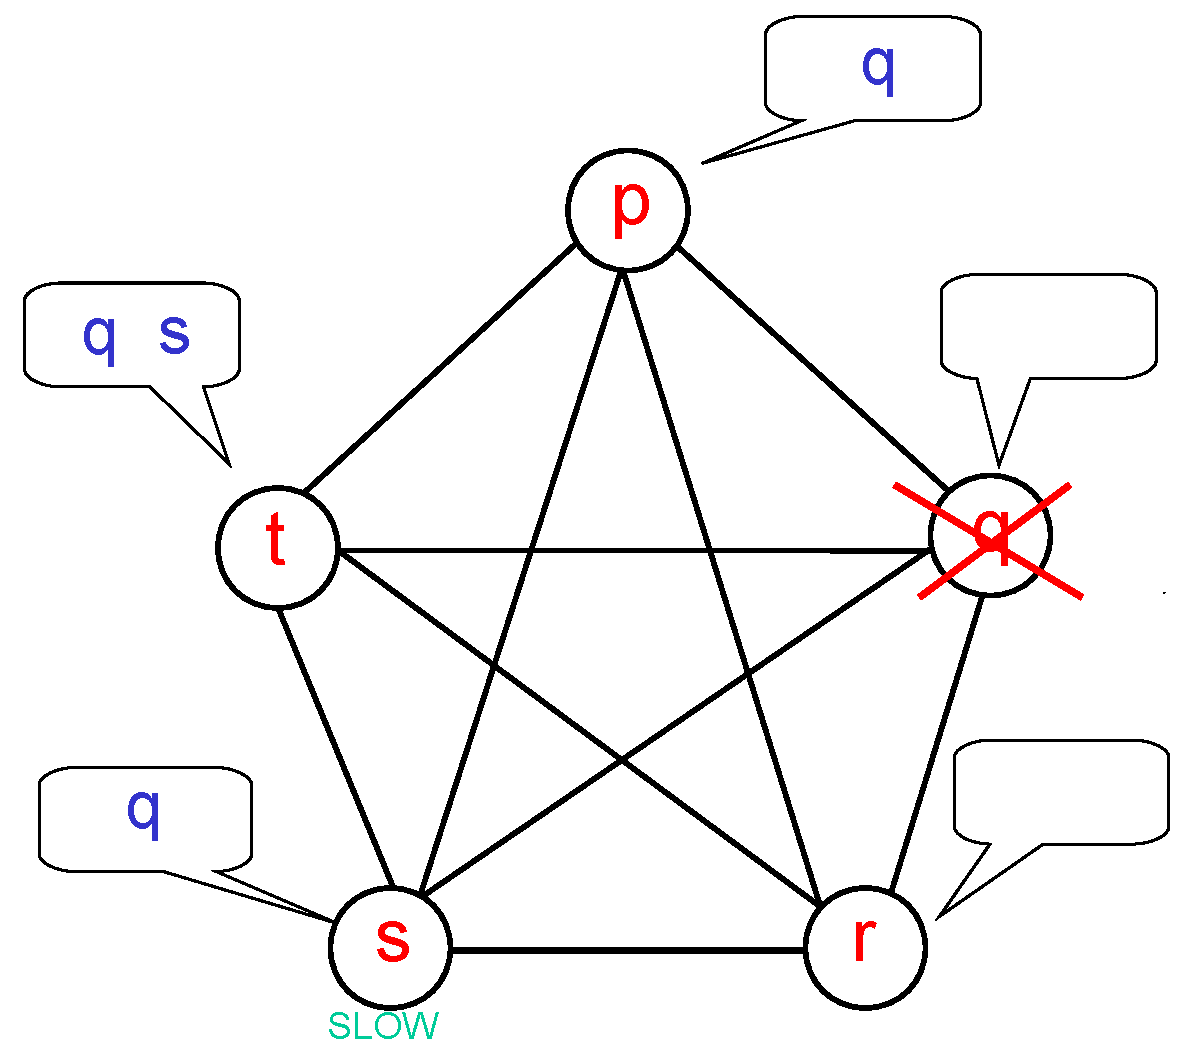
\includegraphics[width=\textwidth]{figs/07/fd}
\end{figure}

\end{column}
\end{columns}

\end{overprint}
\end{frame}

% \begin{frame}{Introduction to FD}
% 
% \begin{definition}[Failure detector]
% A \alert{distributed oracle} whose task is to provide processes with \alert{hints} about which other processes
% are up (operational) or down (crashed)
% \end{definition}
% 
% 
% \end{frame}



\begin{frame}{Failure detectors}

\structure{If they are unreliable, why using failure detectors?}

\BIL
\item Defined by abstract properties
\BI
\item Not defined in term of a specific implementation
\EI
\item Modular decomposition
\BI
\item We show correctness assuming only abstract properties
\item Any FD implementation can be used!
\item Protocols are not expressed in term of low-level parameters
\EI
\EIL

\end{frame}

\begin{frame}{Failure detectors}
	
\structure{Problem}:

Which is the “weakest” failure detector $\mathit{Fd}_{\mathit{min}}(P)$ that
can be used to solve problem $P$ in an asynchronous system?

\bigskip
\structure{From a theoretical point of view}:
\BI
\item Necessary and sufficient conditions
\EI

\bigskip
\structure{Practical considerations}: 
\BI
\item To solve $P$ we need a system where $\mathit{Fd}_{\mathit{min}}(P)$ can be implemented
\item It allows us to determine if problem $P_1$ is “more difficult” than $P_2$
\EI

\end{frame}

\begin{frame}{History}
	
\begin{Bib}
\BIL
\item \bibentry{ct96} 
\item \bibentry{cht96}
\item \bibentry{MR99}
\EIL
\end{Bib}
\end{frame}


\subsection{Specification}

\begin{frame}{Formal definitions (1)}

\begin{definition}[Time]
\BI
\item To simplify the presentation, we assume the existence of a discrete
global clock (not accessible by processes)
\item Let ${\cal T} = \mathbb{N}$ be the \alert{set of clock ticks}
\EI
\end{definition}

\begin{definition}[Failure pattern]
A \alert{failure pattern} is a function $F: {\cal T} \Rightarrow 2^\Pi$,
where $F(t)$ denotes the set of processes that have crashed through time $t$
\BI
\item $\forall t \in {\cal T}: F(t) \subseteq F(t+1)$ (no recovery)
\EI
\end{definition}

\end{frame}

\begin{frame}{Formal definitions (2)}

\begin{definition}{Correct, crashed set}
\BI
\item $\Crashed(F) = \bigcup_{t \in {\cal T}} F(t)$ (\alert{Crashed set})
\item $\Correct(F) = \Pi - \Crashed(F)$ (\alert{Correct set}) 
\item A process is \alert{correct} if belongs to $\Correct(F)$, otherwise is \alert{faulty}
\EI
\end{definition}


\begin{definition}[Failure detector history]
A \alert{failure detector history} is a function $H: \Pi \times {\cal T} \rightarrow 2^\Pi$,
where $H(p,t)$ is the output of the failure detector of process $p$ at time $t$
\BI
\item If $q \in H(p, t)$, we say that $p$ \alert{suspects} $q$ at time $t$ in $H$
\EI
\end{definition}	
	
\end{frame}


\begin{frame}{Completeness}
	
\begin{definition}[Strong Completeness]
Eventually, every faulty process is permanently suspected by \alert{every} correct process.	
\[
\forall F, \forall H, \exists t \in {\cal T}, \forall p \in \Crashed(F), \alert{\forall q} \in \Correct(F), \forall t' \geq t : p \in H(q,t')
\]
\end{definition}
	
\begin{definition}[Weak Completeness]
Eventually, every faulty process permanently suspected by \alert{some} correct process.	
\[
\forall F, \forall H, \exists t \in {\cal T}, \forall p \in \Crashed(F), \alert{\exists q} \in \Correct(F), \forall t' \geq t : p \in H(q,t')
\]
\end{definition}
	
\bigskip
\structure{Motivation behind Weak Completeness}

We do not want every process “to ping” all other processes continuously

\end{frame}
 	
\begin{frame}{Accuracy (1)}

\begin{definition}[Strong Accuracy]
\alert{Every} correct process is never suspected.
\[
\forall F, \forall H, \forall t \in {\cal T}, \alert{\forall p} \in \Correct(F), \forall q : p \notin H(q, t)
\]
\end{definition}

\begin{definition}[Weak Accuracy]
\alert{Some} correct process is never suspected.
\[
\forall F, \forall H, \forall t \in {\cal T},\alert{ \exists p} \in \Correct(F), \forall q : p \notin H(q, t)
\]
\end{definition}
	
	
\end{frame}

\begin{frame}{Accuracy (2)}

\begin{definition}[Eventual Strong Accuracy]
There is a time after which \alert{every} correct process is not suspected by any correct process.
\[
\forall F, \forall H, \exists t \in {\cal T}, \forall t \geq t', \alert{\forall p} \in \Correct(F), \forall q \in \Correct(F): p \notin  H(q,t')
\]
\end{definition}

\begin{definition}[Eventual Weak Accuracy]
There is a time after which \alert{some} correct process is never suspected by any correct process.
\[
\forall F, \forall H, \exists t \in {\cal T}, \forall t \geq t', \alert{\exists p} \in \Correct(F), \forall q \in \Correct(F): p \notin  H(q,t')
\]
\end{definition}
	
	
\end{frame}

\begin{frame}{Failure Detector Classes}

\begin{table}
\begin{tabular}{|l|c|c|c|c|}
%\begin{tabular*}{\textwidth}{@{\extracolsep{\fill}} | l | c | c | c | c |}
%\begin{tabular}{|p{3cm}|p{2cm}|p{2cm}|p{2cm}|p{2cm}|}
\hline
& \multicolumn{4}{|c|}{Accuracy} \\ \cline{2-5}
& \makebox[1.9cm]{Strong} & \makebox[1.9cm]{Weak} & \makebox[1.9cm]{Ev. Strong} & \makebox[1.9cm]{Ev. Weak} \\
\hline
Strong & Perfect  & Strong  & Ev. Perfect & Ev. Strong  \\
Completeness & \alert{$P$} & \alert{$S$} & \alert{$\diamond P$} & \alert{$\diamond S$} \\
\hline
Weak  & & Weak  & & Ev. Weak   \\
Completeness & & \alert{$W$} & & \alert{$\diamond W$} \\
\hline
\end{tabular}
\end{table}

\end{frame}

\subsection{Reductions}

\begin{frame}{Reductions}
	
\begin{definition}[Reduction]
We say that an algorithm $T_{D \rightarrow E}$ is a \alert{reduction} from $D$ to $E$ if it transforms 
a failure detector of class $D$ into a failure detector of class $E$, and we write $D \geq E$.
\end{definition}

\structure{Some easy reductions}:
\begin{figure}
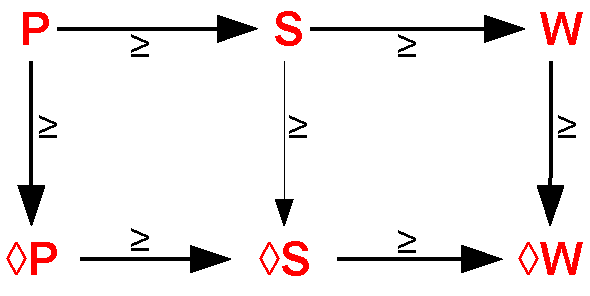
\includegraphics[width=0.6\textwidth]{figs/07/reductions}
\end{figure}

\end{frame}

\begin{frame}{From Weak Completeness to Strong Completeness}

\begin{Procedure}
\caption{Reduction from class $D$ to class $E$, executed by process $p_i$}	
	
\UPON{initialization}{
  $\Suspected^E_i \gets \emptyset$\;
}
\BlankLine
\REPEAT{periodically}{
  $\bbroadcast(\langle \SUSPECT, \Suspected^D_i \rangle)$\;
}
\BlankLine
\UPON{$\bdeliver(\langle \SUSPECT, S \rangle)$ \FROM $p_j$}{
  $\Suspected^E_i \gets \Suspected^E_i \cup S - \{ p_i, p_j \}$\;
}
\end{Procedure}	

\structure{Using this reduction, we can show that}:
\BI
\item $\diamond W \geq \diamond S$, so $\diamond W \equiv \diamond S$
\item $W \geq S$, so $W \equiv S$
\EI

\end{frame}

%%%%%%%%%%%%%%%%%%%%%%%%%%%%%%%%%%%%%%%%%%%%%%%%%%%%%%%%%%%%%%%%%%%%%%%%

\section{Reliable Broadcast}

\begin{frame}{Reliable Broadcast Recap}
	
\structure{Reliable Broadcast}

\BI
  \item Implementable with process failures and message omissions
  \item Proposed implementation: flooding, $O(n^2)$ messages
\EI

\bigskip
\structure{Uniform Reliable Broadcast}

\BI
\item Implementable with process failures and no message omissions
\item Same implementation (different assumptions)
\EI

\bigskip
\structure{Message complexity}

\BI
\item Conservative protocol: many messages in the absence of failures
\item Can we do better than that?
\item We apply failure detectors
\EI

\end{frame}

\begin{frame}[shrink=10]{}


\begin{Procedure}
\caption{Reliable broadcast protocol based on $\diamond P$ executed by $p$}
\UPON{initialization}{
  $\Set\ \Delivered \gets \Set\langle \Message \rangle$~~~~~~~~~\Comment*[f]{Msgs already delivered}\;
  $\Map\ \From \gets \NEW\ \Map\langle \Process, \Set\rangle()$\Comment*[f]{Msgs sent from processes}\;

}
\BlankLine
\UPON{$\rbroadcast(m)$}{
  \SEND $\langle m, p \rangle$ \TO $\Pi$\;
}
\BlankLine
\UPON{$q \in {\diamond}P.\Suspect()$}{
  \ForEach{$m \in \From[q]$}{
    \SEND $\langle m, q \rangle$ to $\Pi$\;
  }
}
\UPON{$\RECEIVE(\langle m, s \rangle)$}{
  $\From[s] \gets \From[s] \cup \{ m \}$\;
  \If{\NOT $m \in \Delivered$}{
    $\rdeliver(m)$\;
    $\Delivered \gets \Delivered \cup \{ m \}$\;
    \If{$s \in {\diamond}P.\Suspect()$}{
      \SEND $\langle m, s \rangle$ to $\Pi$\;
    }
  }
}
\end{Procedure}

\end{frame}

\begin{frame}{Reliable Broadcast with $\diamond P$ -- Scenario 1}
	
\begin{figure}
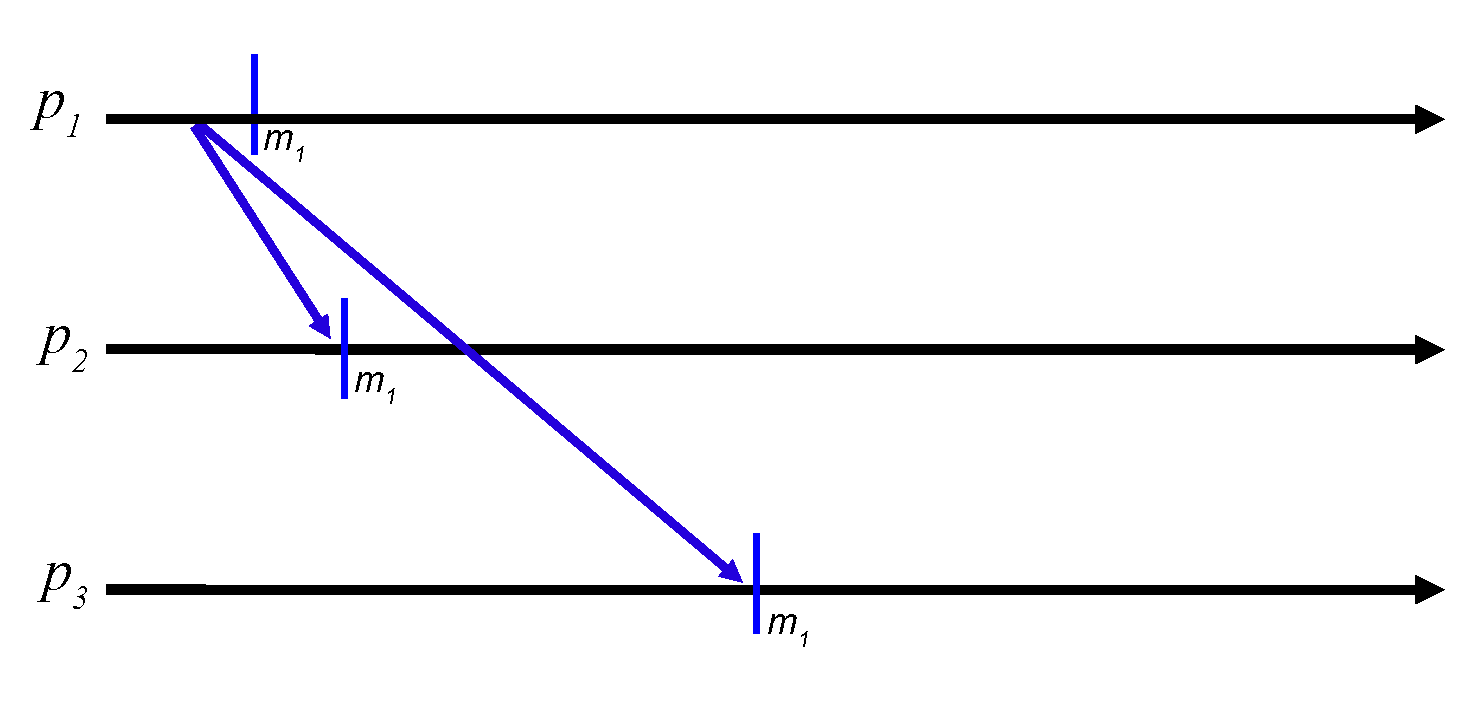
\includegraphics[width=\textwidth]{figs/07/rb-diamond1}
\end{figure}
	
\end{frame}

\begin{frame}{Reliable Broadcast with $\diamond P$ -- Scenario 2}
	
\begin{figure}
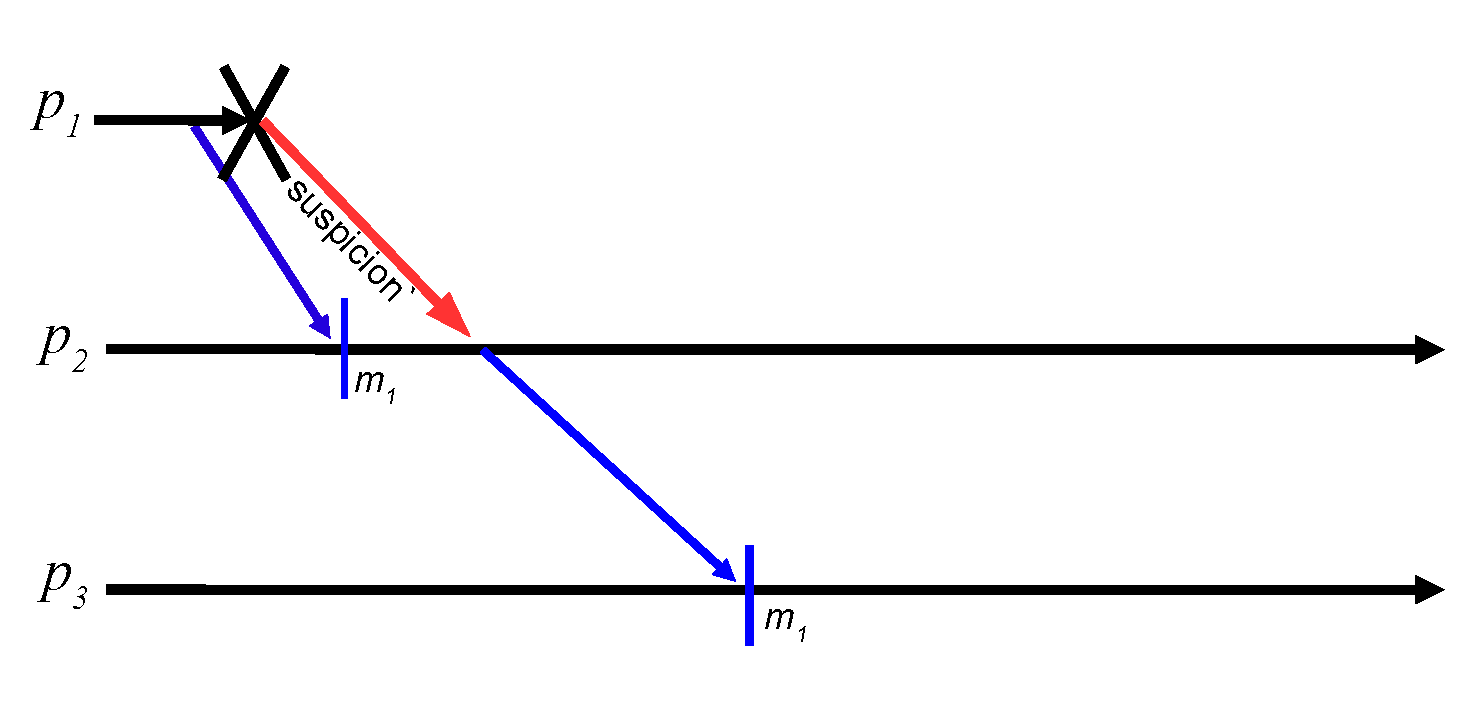
\includegraphics[width=\textwidth]{figs/07/rb-diamond2}
\end{figure}

\end{frame}
	
\begin{frame}{Reliable Broadcast with $\diamond P$ -- Proof}
\BIL
\item \alert{Uniform Integrity}, \alert{Validity}: As before
\item \alert{Agreement}:\\
Let $p$ be a process that R-delivers a message $m$\\
Let $q$ be another process\\
Let $s = \Sender(m)$; there are two cases\\
\BI
\item Case 1: $s$ is correct -- by Validity of Perfect Channels
\item Case 2: $s$ is faulty -- by Eventual Strong Accuracy
\EI
\EIL

\bigskip
\begin{block}{Comment}
If the failure detector is not accurate, more messages will be sent; but not other adverse effect will occur
\end{block}

\note{
\structure{Proof of Reliable Broadcast using $\diamond P$}

By contradiction, let $p$ and $q$ two correct processes such
that $p$ R-delivers a message $m$ that $q$ never R-delivers.

Let $\Sender(m) = s$. There are two cases
\BI
\item $s$ is correct; by Validity of Perfect Channels, 
  $m$ will eventually be received by $q$, that R-deliver it
  (a contradiction)
\item $s$ is faulty; by Eventual Strong Accuracy, $s$ will
  be eventually suspected by all correct process, so also
  by $p$; $p$ will forward the message $m$ to all processes, 
  and by Validity of Perfect Channels $q$ will eventually
  receive it.
\EI

}

\end{frame}	

% \begin{frame}[shrink]{Uniform Reliable Broadcast with $P$}
% 
% \begin{Procedure}
% \caption{Reliable broadcast protocol executed by process $p$}
% \UPON{initialization}{
%   $\Set\langle\Message\rangle\ \Delivered \gets \emptyset$\Comment*[f]{Messages already delivered}\;
%   $\Set\langle\Message\rangle\ \Forward \gets \emptyset$\Comment*[f]{Messages already forwarded}\;
%   $\Map\langle \Message, \Set\rangle\ \Ack \gets \NEW\ \Map\langle \Message, \Set\rangle()$\;
%   ~\Comment*[f]{Acks received for each message}\;
% }
% \BlankLine
% \UPON{$\urbroadcast(m)$}{
%   \SEND $\langle m, p, \Seqn(m) \rangle$ \TO $p$\Comment*[f]{Makes $m$ unique}\;
% }
% \BlankLine
% \UPON{$\receive(m)$}{
%   \lIf{$\Ack[m] = \NIL$}{$\Ack[m] \gets \emptyset$\;}
%   $\Ack[m] \gets \Ack[m] \cup \{ \Sender(m) \}$\;
%   \If{$m \notin \Forward$}{
%     $\Forward \gets \Forward \cup \{ m \}$\;
%     \SEND $m$ \TO $\Pi$\; 
%   }
% }
% \BlankLine
% \UPON{$\exists m \in \Forward : P.\Suspect() \cup \Ack[m] = \Pi \wedge m \notin \Delivered$}{
%   $\Delivered \gets \Delivered \cup \{ m \}$\;
%   $\urdeliver(m)$\;
% }
% 
% \end{Procedure}
% 
% \note{
% \begin{teorema}{Eventual Delivery}
% If a correct process $p$ receive a message $m$, then $p$ eventually UR-delivers $m$. 
% \end{teorema}
% 
% \begin{prova}
% Any process that receives $m$ forwards it to all processes. 
% By the Completeness property of $P$ and Validity property of
% Perfect Channel, there is a time at which $p$ receive $m$ from 
% every correct process and hence R-delivers $m$.
% \end{prova}
% 
% \begin{teorema}{Validity}
% The URB protocol satisfies Validity
% \end{teorema}
% 
% \begin{prova}
% If a correct process $p$ UR-broadcasts a message $m$, then $p$ 
% first send it to all processes, and then receives it: by our lemma, $p$ 
% R-delivers $m$.
% \end{prova}
% 
% \begin{teorema}{Agreement}
% The URB protocol satisfies Agreement.
% \end{teorema}
% 
% \begin{prova}
% Assume some process $p$ R-delivers a message $m$. By Strong Accuracy and
% Completeness, this means that every correct process has sent $m$ to $p$. 
% By our lemma, every correct process will R-deliver $m$. Note: Strong Accuracy is
% needed, otherwise $p$ could R-deliver $m$ without other processes
% R-delivering it.
% \end{prova}
% 
% }
% 
% \end{frame}
% 
% \begin{frame}{Reliable Broadcast with $P$ -- Scenario 1}
% 	
% \begin{figure}
% 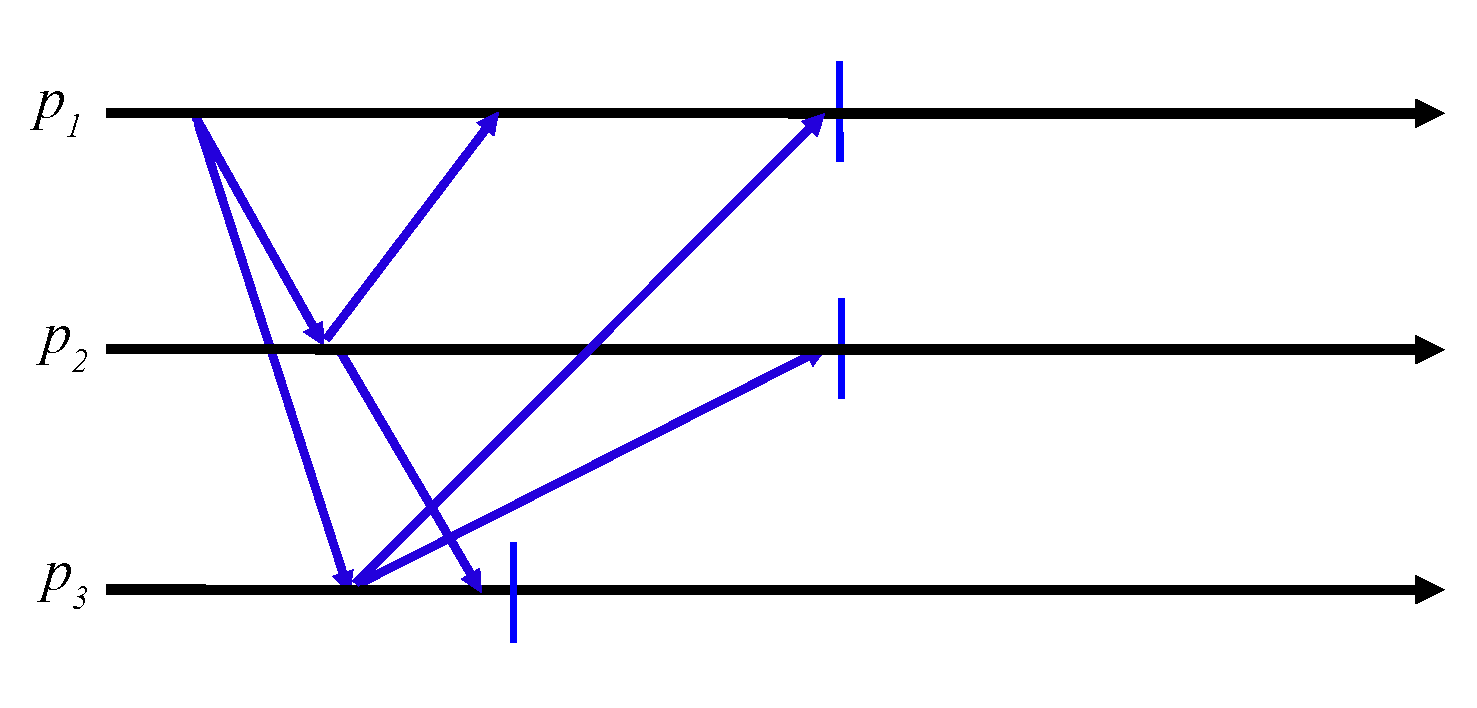
\includegraphics[width=\textwidth]{figs/07/rb-urb-scenario1}
% \end{figure}
% 
% 	
% \end{frame}
% 
% \begin{frame}{Reliable Broadcast with $P$ -- Scenario 1}
% 	
% \begin{figure}
% 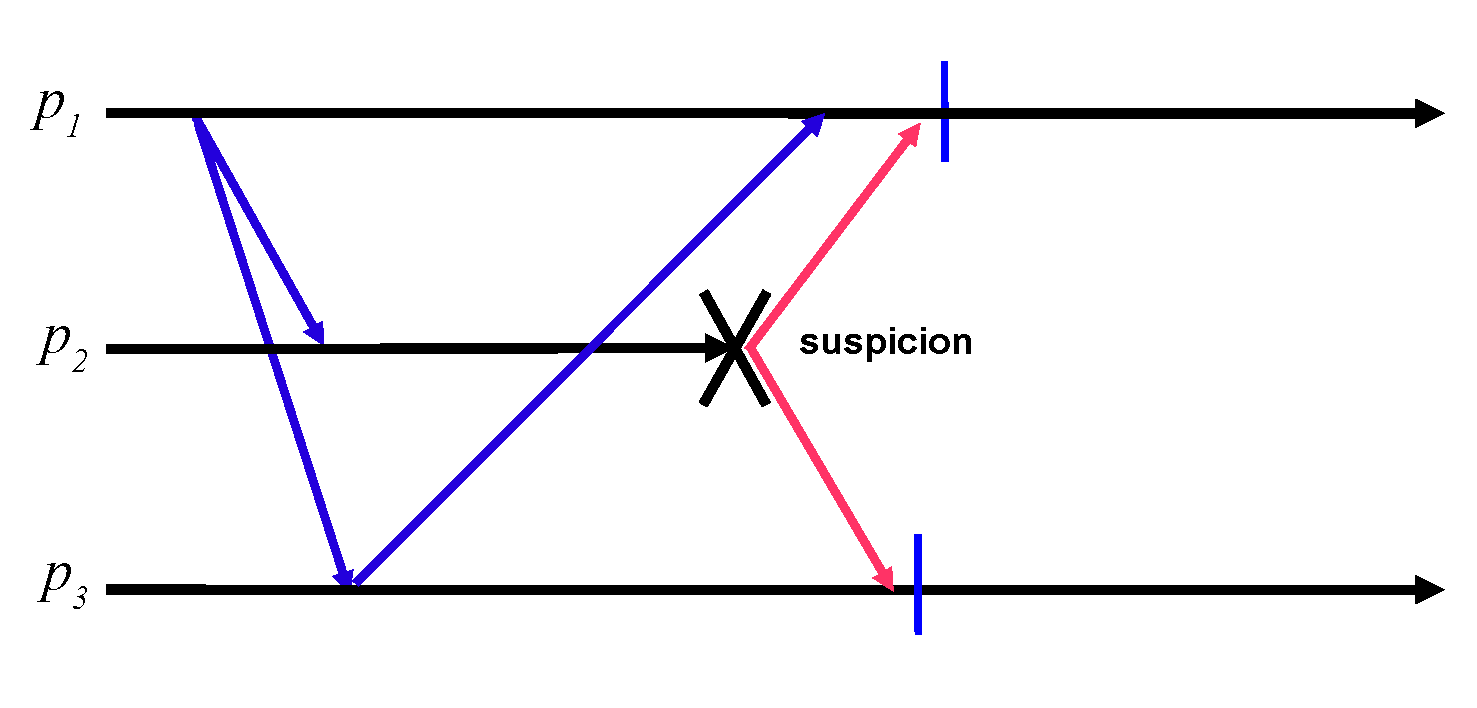
\includegraphics[width=\textwidth]{figs/07/rb-urb-scenario2}
% \end{figure}
% 	
% 
% \end{frame}

\begin{frame}{Reliable Broadcast through FD}

\structure{Reliable Broadcast}

\BIL
\item Can be implemented using a linear number of messages in the absence of failures
\item An Eventually Perfect FD as accurate as possible is required to reduce the number of messages
\EIL

\structure{But...}

\BIL
\item Think what is needed to implement a failure detector!
\EIL



% \structure{Uniform Reliable Broadcast}
% 
% \BIL
% \item A $O(n^2)$ number of message is still needed
% \item Problems of messages losses, asynchrony, failures are “hidden” in the Perfect FD.
% \EIL

\end{frame}

%%%%%%%%%%%%%%%%%%%%%%%%%%%%%%%%%%%%%%%%%%%%%%%%%%%%%%%%%%%%%%%%%%%%%%%%

\section{Consensus}

\subsection{Introduction}

\begin{frame}{Consensus and Failure Detectors}
	
\begin{block}{Problem}
Is perfect failure detection necessary for Consensus? 
\end{block}

\begin{overprint}

\onslide<1|handout:1>
\bigskip
\structure{$\diamond S$ versus Consensus}:

\BIL
\item Initially, it can output arbitrary information
\item But there is a time after which:
\BI
  \item \alert{Every} process that crashes is suspected (completeness)
  \item \alert{Some} process that does not crash is not suspected (accuracy)
\EI
\item When $f < n/2$, $\diamond S$ is necessary and sufficient to solve Consensus
\item Note: $\diamond S \equiv \diamond W$
\EIL	

\onslide<2|handout:2>
\bigskip
\structure{$S$ versus Consensus}:

\BIL
\item It can output arbitrary information about most of the processes
\item But there is at least one correct process which is never suspected
\item When $f < n$, $S$ is necessary and sufficient to solve Consensus
\item Note: $S \equiv W$
\EIL	

\end{overprint}

\end{frame}

\begin{frame}{Rotating coordinators}
	
\begin{columns}
\begin{column}{0.6\textwidth}
\BIL
\item Processes are numbered $0, 1, \ldots, n-1$
\item They execute asynchronous rounds
\item In round $r$, the coordinator
  \BI
  \item corresponds to process $(r \bmod n)$
  \item tries to impose its estimate as the consensus value
  \item succeeds if does not crash and it is not suspected by $\diamond S$
  \EI
\item The protocol described here is based on [Mostéfaoui and Raynal, 1999]
\EIL
\end{column}
\begin{column}{0.4\textwidth}
	\begin{figure}
		\begin{overprint}
			\onslide<1|handout:0>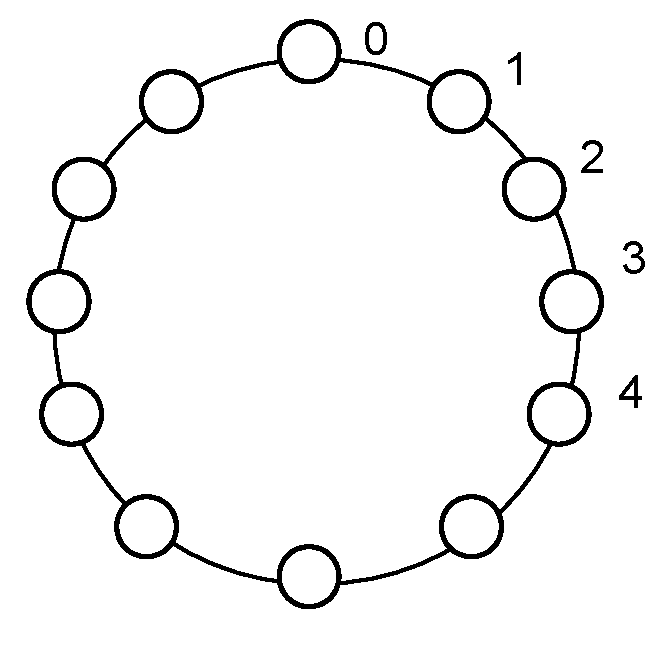
\includegraphics[width=\textwidth]{figs/07/rotating0}
			\onslide<2|handout:0>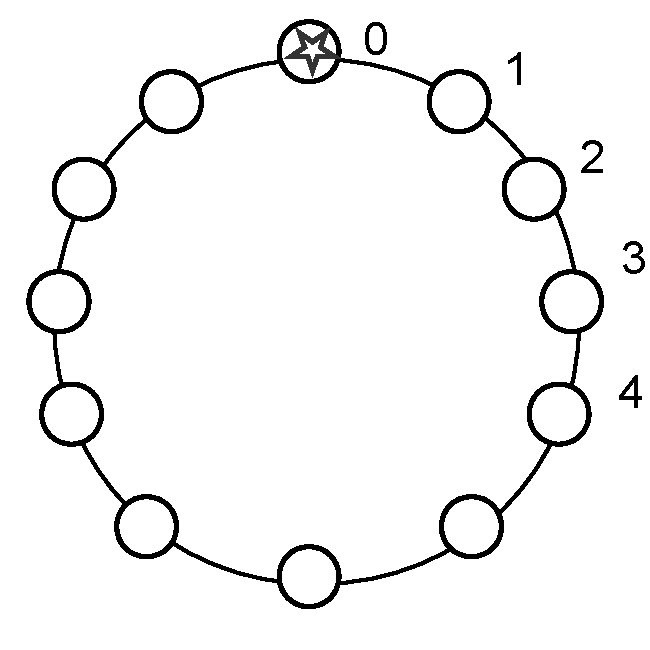
\includegraphics[width=\textwidth]{figs/07/rotating1}
			\onslide<3|handout:0>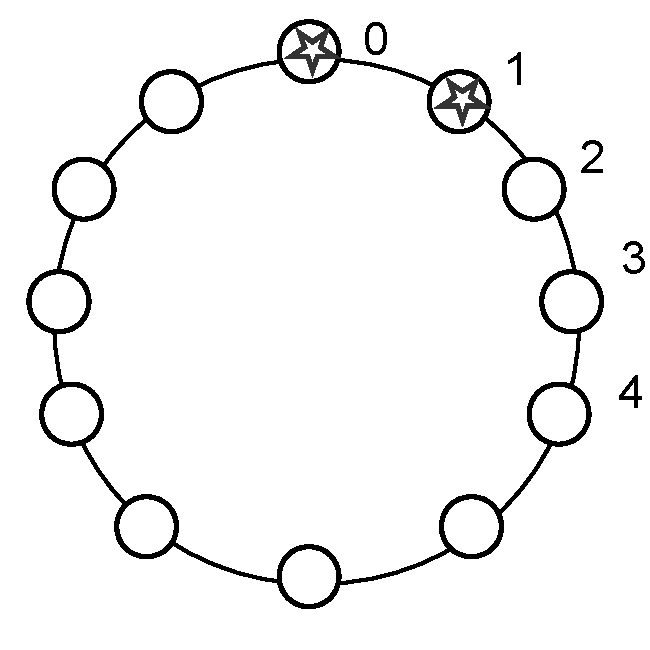
\includegraphics[width=\textwidth]{figs/07/rotating2}
			\onslide<4|handout:0>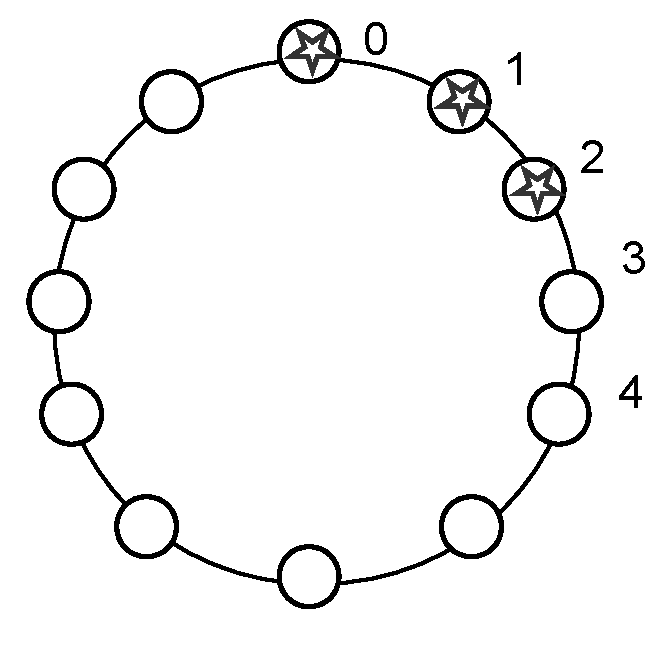
\includegraphics[width=\textwidth]{figs/07/rotating3}
			\onslide<5|handout:1>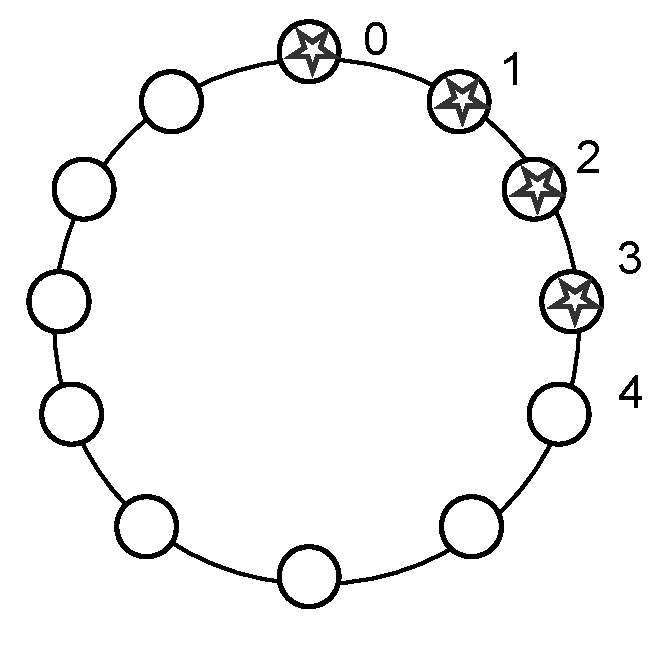
\includegraphics[width=\textwidth]{figs/07/rotating4}
		\end{overprint}
	\end{figure}
\end{column}
\end{columns}

\end{frame}

\subsection{Algorithms}

\begin{frame}[shrink=15]{}
	
	
\begin{Procedure}	
\caption{Consensus Algorithm based on $\diamond S$ executed by process $p_i$}
\UPON{$\Propose(v_i)$}{
  \INTEGER $r \gets 0$\Comment*[f]{Round}\;
  \INTEGER $\Est \gets v_i$\Comment*[f]{Estimate}\;
  \BOOLEAN $\Decided \gets \FALSE$\;
  \BOOLEAN $\Stop \gets \FALSE$\;
}
\BlankLine
\uWHILE{\NOT $\Stop$}{
  \INTEGER $c \gets r \bmod n$\Comment*[f]{Coordinator}\;
  $r \gets r+1$\;
  \BlankLine
  \alert{\{ Phase 1 of round $r$; from $p_c$ to all \}}\;
  \BlankLine
  \If{$i=c$}{
    $\bbroadcast(\langle \PHASEA, r, \Est, p_i \rangle)$\;
  }
  \lnlset{InResR}{1}\WAIT $\bdeliver(\langle \PHASEA, r, v, p_c \rangle)$ \OR $p_c \in \Suspected_i^{\diamond S}$\;
  \eIf{$p_c \in \Suspected_i$}{
    $\Aux \gets\ ?$\;
  }{
    $\Aux \gets v$\;
  }
}
\end{Procedure}	

\end{frame}

\begin{frame}[shrink=15]{}
	
	
\begin{Procedure}	
\caption{Consensus Algorithm based on $\diamond S$ executed by process $p_i$}
\vspace{-12pt}
\UNVISIBLE{}{
  \alert{\{ Phase 2 of round $r$; from all to all \}}\;
  \BlankLine
  $\bbroadcast(\langle \PHASEB, r, \Aux, p_i \rangle)$\;
  $\Set\ \Rec \gets \emptyset$\Comment*[f]{Received values}\;
  $\Set\ \Proc \gets \emptyset$~~~\Comment*[f]{Replying processes}\;
  \While{$|\Proc| \leq \lfloor n/2 \rfloor$}{
    \lnlset{InResR}{2}\WAIT $\bdeliver(\langle \PHASEB, r, v , p_j \rangle)$\;
    $\Rec \gets \Rec \cup \{ v \}$\;
    $\Proc \gets \Proc \cup \{ p_j \}$\;
  }
  \lIf{$\Rec = \makebox[0.9cm]{$\{ v \}$}$}{$\Est \gets v$; $\bbroadcast(\langle \DECIDE, v \rangle)$; $\Stop \gets \TRUE$}
  \lIf{$\Rec = \makebox[0.9cm]{$\{ v, ? \}$}$}{$\Est \gets v$}
  \lIf{$\Rec = \makebox[0.9cm]{$\{ ? \}$}$}{do nothing}
}
\BlankLine
\UPON{$\bdeliver(\langle \DECIDE, v \rangle)$}{
  \If{\NOT $\Decided$}{
    $\bbroadcast(\langle \DECIDE, v \rangle)$\;
  	$\Decide(v)$\;
    $\Decided \gets \TRUE$\;
  }
}
\end{Procedure}	

\end{frame}

\begin{frame}{Proof of correctness -- Termination}

\begin{proof}[Termination]	
\BI
\item \WAIT \#1: With $\diamond S$, no process blocks forever waiting for a message 
  from a dead coordinator
\item \WAIT \#2: Given that $f<n/2$, eventually every node will receive more
than $\lfloor n/2 \rfloor$ messages and will exit from Phase 2
\item Thanks to $\diamond S$, eventually some correct process $p_c$ is not falsely 
  suspected. When $p_c$ becomes the coordinator, every correct process receives $c$'s 
  estimate and decides.
\EI
\end{proof}

\end{frame}


\begin{frame}{Proof of correctness -- Agreement}

\note{
\BI
\item When a process decides $v$, it has received a majority of messages
containing $v$
\item There is a majority of correct nodes
\item The intersection of these majorities is not empty
\item Every correct process will receive at least one $v$ from such process
\EI
}

\begin{figure}
	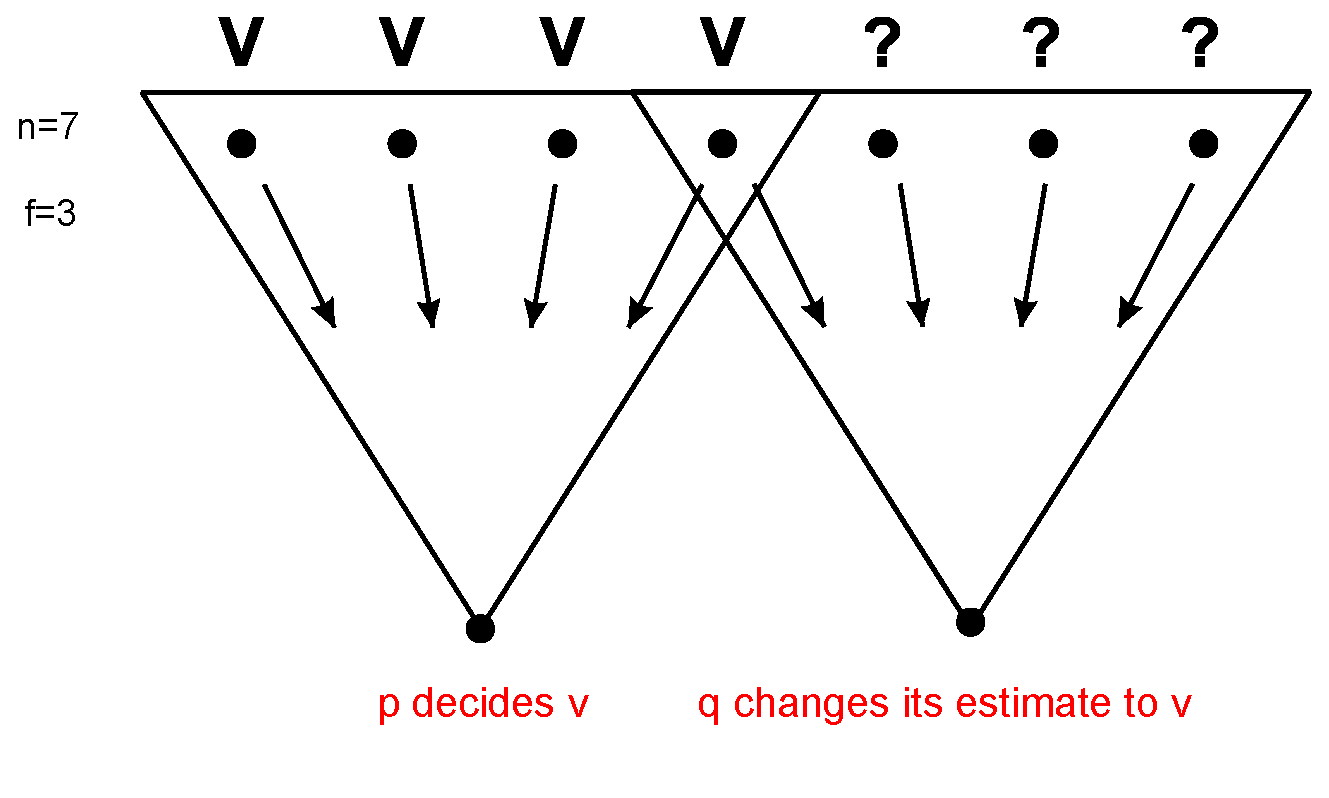
\includegraphics[width=\textwidth]{figs/07/agreement}
\end{figure}

\end{frame}

\begin{frame}[shrink=15]{}
	
	
\begin{Procedure}	
\caption{Consensus Algorithm based on $S$  executed by process $p_i$}
\UPON{$\Propose(v_i)$}{
  \INTEGER $r \gets 0$\Comment*[f]{Round}\;
  \INTEGER $\Est \gets v_i$\Comment*[f]{Estimate}\;
  \BOOLEAN $\Decided \gets \FALSE$\;
  \BOOLEAN $\Stop \gets \FALSE$\;
}
\BlankLine
\uWHILE{\NOT $\Stop$}{
  \INTEGER $c \gets r \bmod n$\Comment*[f]{Coordinator}\;
  $r \gets r+1$\;
  \BlankLine
  \alert{\{ Phase 1 of round $r$; from $p_c$ to all \}}\;  
  \BlankLine
  \If{$i=c$}{
    $\bbroadcast(\langle \PHASEA, r, \Est, p_i \rangle)$\;
  }
  \lnlset{InResR}{1}\WAIT $\bdeliver(\langle \PHASEA, r, v, p_c \rangle)$ \OR $p_c \in \Suspected_i^S$\;
  \eIf{$p_c \in \Suspected_i$}{
    $\Aux \gets\ ?$\;
  }{
    $\Aux \gets v$\;
  }
}
\end{Procedure}	

\end{frame}

\begin{frame}[shrink=15]{}
	
	
\begin{Procedure}	
\caption{Consensus Algorithm based on $S$  executed by process $p_i$}
\vspace{-12pt}
\UNVISIBLE{}{
  \alert{\{ Phase 2 of round $r$; from all to all \}}\;
  \BlankLine
  $\bbroadcast(\langle \PHASEB, r, \Aux, p_i \rangle)$\;
  $\Set\ \Rec \gets \emptyset$\Comment*[f]{Received values}\;
  $\Set\ \Proc \gets \emptyset$~~~\Comment*[f]{Replying processes}\;
  \While(\Comment*[f]{Was: \color{blue}{$|\Proc| < n/2$}}){\color{blue}{$\Proc \cup \Suspected_i^S \neq \Pi$}}{
    \lnlset{InResR}{2}\WAIT $\bdeliver(\langle \PHASEB, r, v , p_j \rangle)$\;
    $\Rec \gets \Rec \cup \{ v \}$\;
    $\Proc \gets \Proc \cup \{ p_j \}$\;
  }
  \lIf{$\Rec = \makebox[0.9cm]{$\{ v \}$}$}{$\Est \gets v$; $\bbroadcast(\langle \DECIDE, v \rangle)$; $\Stop \gets \TRUE$}
  \lIf{$\Rec = \makebox[0.9cm]{$\{ v, ? \}$}$}{$\Est \gets v$}
  \lIf{$\Rec = \makebox[0.9cm]{$\{ ? \}$}$}{do nothing}
}
\BlankLine
\UPON{$\bdeliver(\langle \DECIDE, v \rangle)$}{
  \If{\NOT $\Decided$}{
    $\bbroadcast(\langle \DECIDE, v \rangle)$\;
  	$\Decide(v)$\;
    $\Decided \gets \TRUE$\;
  }
}
\end{Procedure}	

\note{
TODO: Scrivere due parole sulla dimostrazione.
}

\end{frame}

\subsection{Discussion}

\begin{frame}{What if the FD misbehaves}

\BIL
\item Accuracy can be not satisfied
\BI 
\item Consensus algorithm remains always safe
\item It is also live -- during “good” FD periods
\EI
\item Completeness is always satisfied
\EIL
	
\begin{figure}
	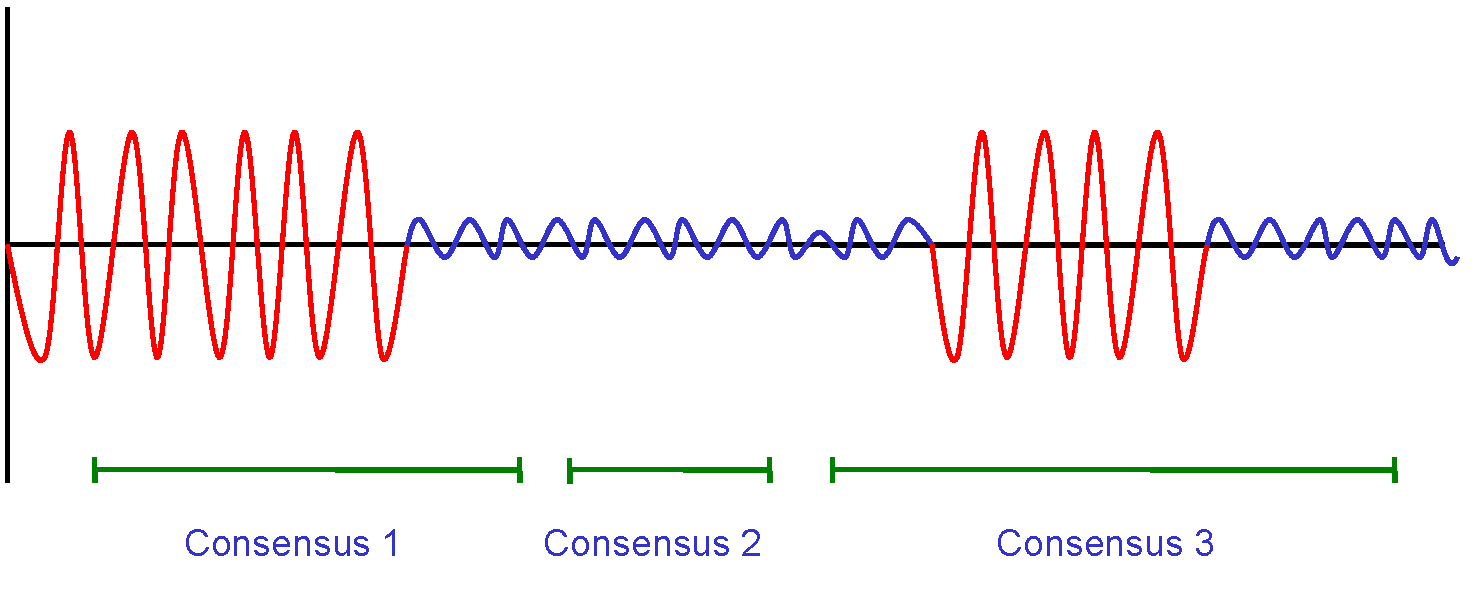
\includegraphics[width=\textwidth]{figs/07/goodbadtimes}
\end{figure}

\end{frame}

\begin{frame}{Indulgent algorithms}

\begin{definition}[Indulgent algorithms]
\BI
\item Never violate the safety property
\item If the FD is not accurate, they do not terminate
\item Require “stable” periods in order to terminate
\EI
\end{definition}

\bigskip
\structure{The protocol just shown is an indulgent algorithm}

\bigskip
\begin{Bib}
\BI
\item \bibentry{Gue00}
\EI
\end{Bib}

\end{frame}


\begin{frame}{Failure detectors as an abstraction}

\structure{Some advantages}

\BIL
\item Increases the modularity and portability of algorithms
\item Suggests why Consensus is not so difficult in practice
\item Determines minimal info about failures to solve consensus
\item Encapsulates various models of partial synchrony
\EIL

\end{frame}

\begin{frame}{Broadening the applicability of  FDs}
	
\structure{Other models}
\BI
\item Crashes + Link failures (fair links)
\item Network partitioning
\item Crash/Recovery
\item Byzantine (arbitrary) failures
\item FDs + Randomization
\EI

\bigskip
\structure{Other problems}
\BI
\item Atomic Commitment
\item Group Membership
\item Leader Election
\item Reliable Broadcast \qquad $\checkmark$
\EI

\end{frame}

\begin{frame}[shrink=3]{From theory to practice}
	
\BIL
\item \alert{FD implementation needs to be message-efficient}:
	\BI
	\item FDs with linear message complexity (ring, hierarchical, gossip) 
	\EI
\item \alert{“Eventual” guarantees are not sufficient}:
	\BI
	\item FDs with Quality-of-Service guarantees
	\EI
\item \alert{Failure detection should be easily available}:
	\BI
	\item Shared FD service (with QoS guarantees)
	\EI
\EIL

\bigskip
\begin{Bib}
\BI
\item \bibentry{fd-gossip}
\item \bibentry{fd-qos}
\EI
\end{Bib}

\note{When speaking about shared FD services, make a note back to the 
discussion about implementing Reliable Broadcast with or without a FD}

\end{frame}

\section{Randomization}

\subsection{Ben-Or protocol}

\begin{frame}{Another approach: randomization}

\BI
\item First protocol to achieve \alert{binary} Consensus with probabilistic termination in an asynchronous model 
\item The protocol is $f$-correct - tolerates up to $f$ crash failures, with $f < n/2$ 
\item Expected time: $O(2^{2n})$ phases to converge
\EI

\bigskip
\begin{Bib}
\BI
\item \bibentry{ben-or83}
\EI
\end{Bib}

\end{frame}

\begin{frame}{Ben-Or's Algorithm}

\BIL	
\item Operates in rounds, each round has two phases:
\BI
\item \alert{Report phase} – each process transmits its value, and waits to hear from other processes
\item \alert{Decision phase} – if majority found, take its value; otherwise, flip a coin to change the local value
\EI

\item The idea:
\BI
\item If enough processes detected the majority, decide
\item If I know that someone detected majority, switch to the majority’s value
\item Otherwise, flip a coin; eventually, a majority of correct processes will flip in the same way
\EI

\EIL
\end{frame}


\begin{frame}[shrink=20]{}

\begin{Procedure}	
\caption{Ben-Or's Algorithm executed by process $p_i$}
\UPON{$\Propose(v_i)$}{
  \INTEGER $r \gets 0$\Comment*[f]{Round}\;
  \INTEGER $\Est \gets v_i$\Comment*[f]{Estimate}\;
}
\BlankLine
\While{\TRUE}{
  $r \gets r+1$\;
  $\bbroadcast(\langle \REPORT, r, \Est \rangle)$\;
  \WAIT to deliver more than $n-f$ $\langle \REPORT, r, * \rangle$ messages\;
  \eIf{delivered more than $n/2$ $\langle \REPORT, r, v \rangle$ messages with the same value $v$}{
    $\bbroadcast(\langle \PROPOSAL, r, v \rangle)$\;
  }{
    $\bbroadcast(\langle \PROPOSAL, r, ? \rangle)$\;
  }
  \WAIT to deliver more than $n-f$ $\langle \PROPOSAL, r, * \rangle$ messages\;
  \eIf{delivered a $\langle \PROPOSAL, r, v \rangle$ with $v$ with $v \neq ?$}{
    $\Est \gets v$\;
  }{
    $\Est \gets \Random(\{ 0, 1 \})$\;
  }
  \If{delivered more than $f$ $\langle \PROPOSAL, r, v \rangle$ with $v$ with $v \neq ?$}{
    $\Decide(v)$\;
  }
}
\end{Procedure}

\end{frame}

\begin{frame}{The algorithm}
\BIL
\item Based on the original version of Ben-Or
\item It never stops; once decided, it keeps deciding the same value
\item It is easy to transform it in an algorithm that stops one round after
the one in which the decision has been taken
\EIL
\end{frame}

\begin{frame}{Proof of correctness}
	
\begin{proof}[Uniform Agreement]
\BIL
\item At most one value can receive majority in the first phase of a round
\item If some process sees $f+1$ $\langle \PROPOSAL, r, v \neq ? \rangle$, then:
\BI 
\item every process sees at least one $\langle \PROPOSAL, r, v \neq ? \rangle$ message
\EI
\item if every process sees at least one $\langle \PROPOSAL, r, v \neq ? \rangle$ message, then
\BI 
\item every process changes its estimate to $v$
\item every process reports $v$ in the first phase of round $r+1$
\EI
\item If every process reports $v$ in the first phase of round $r+1$,
\BI
\item every process decides $v$ in the second phase of round $r+1$
\EI
\EIL
\end{proof}

\end{frame}


\begin{frame}{Proof of correctness}
\begin{proof}[Validity]
\BIL
\item If there are two distinct values at the beginning, one of them will be chosen
\item Otherwise, if all processes report their common value $v$ at round $0$, then:
\BI
  \item all processes send $\langle \PROPOSAL, 0, v \rangle$
  \item all processes decide on the second phase of round $0$
\EI
\EIL
\end{proof}
\end{frame}

\begin{frame}{Proof of correctness}
	
\begin{proof}[Termination]
\BIL
\item If no process sees the majority value, then they all will flip coins, and start everything again
\item Eventually a majority among the correct processes flips the same random value
	\BI
	\item The correct processes will observe the majority value.
	\item The correct processes will propagate $\PROPOSAL$ messages, containing the majority value
	\EI
\item Correct processes will receive the $\PROPOSAL$ messages, and the protocol finishes
\EIL
\end{proof}

\end{frame}

\section{Hybrid approach}

\begin{frame}{Hybrid approach}
	
\BIL
\item We can combine
	\BI
	\item Failure Detectors
	\item Randomized approach
	\EI
\item Advantages:
	\BI
	\item Deterministic termination if FD is accurate (“good periods”)
	\item Probabilistic termination otherwise (“bad periods”)
	\EI
\item Oracles available at each process
	\BI
	\item FD-oracle: Failure detector $\diamond S$
	\item R-oracle: Random coin-flip
	\EI
\EIL	


\begin{Bib}
\BI
\item \bibentry{hybrid-consensus}
\EI
\end{Bib}
	
\end{frame}




%%%%%%%%%%%%%%%%%%%%%%%%%%%%%%%%%%%%%%%%%%%%%%%%%%%%%%%%%%%%%%%%%%%%%%%%

%\section{Bibliography}

\begin{PlainFrame}{Reading material}

\begin{Bib}
\BI
\item \bibentry{ct96}
\item \bibentry{MR99}
\EI
\end{Bib}
\end{PlainFrame}


\end{document}